\documentclass[../main.tex]{subfiles}
\begin{document}
\graphicspath{{figures/}{task4/figures/}}

\subsection{Task 4: Game Title Detection (macro F1)}
\label{sec:t4}

\subsubsection{Problem and Data}

Task 4 asks for the game title shown in a single gameplay screenshot. There are five titles: 0~7-11 Knights, 1~FiveN, 2~Free Fried, 3~PUBE and 4~Roblock. The metric is \textbf{macro F1}, the unweighted mean of the five per-class F1 scores, so the small classes count as much as the large one.

The training set holds 31,546 labelled images and the test set 25,889 images. \texttt{train.csv} has the columns \texttt{id}, \texttt{file\_name} and \texttt{label}. Every image is an RGB JPEG of $230\times120$ pixels (centre-cropped from $256\times144$, according to the data card). The images come from live streams, player submissions, community forums and support tickets, and cover different maps, game phases and UI states. The submission is one predicted label per test image.

\subsubsection{EDA Findings}

All figures in this section use \emph{training} images only. We looked at the class balance, the images themselves, simple colour statistics, and how repetitive the training scenes are.

\paragraph{Class balance.}

\begin{figure}[H]
\centering
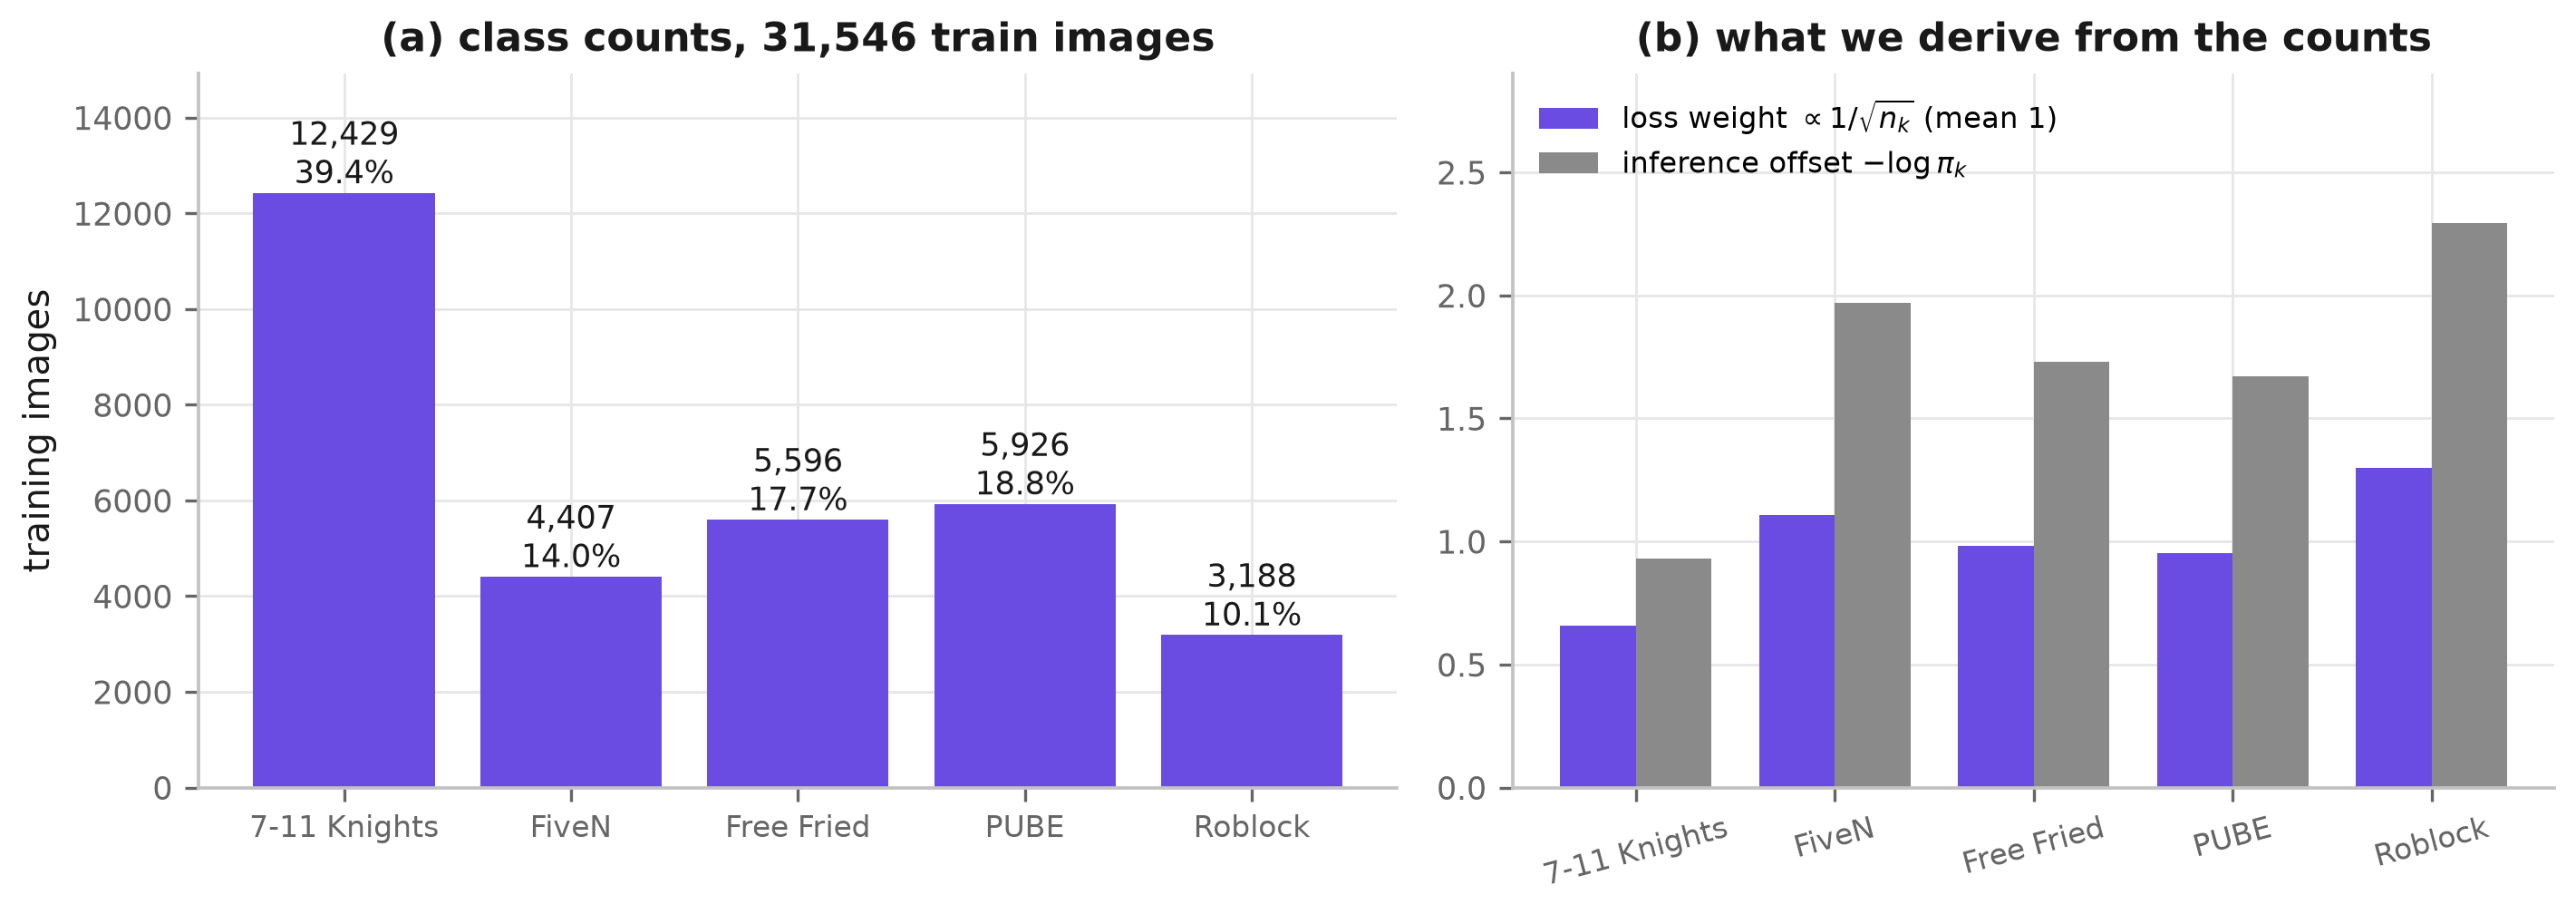
\includegraphics[width=\linewidth,height=0.32\textheight,keepaspectratio]{fig_t4_class_balance.png}
\caption{(a) Training images per title. (b) The two quantities we derive from the counts: the mild loss weight $1/\sqrt{n_k}$ and the logit offset $-\log\pi_k$ used at inference. 7-11 Knights has about four times as many images as Roblock.}
\label{fig:t4-balance}
\end{figure}

Figure~\ref{fig:t4-balance}a shows 39.4\% of the images in 7-11 Knights and 10.1\% in Roblock. Because macro F1 gives each title the same weight, a model trained with plain cross-entropy drifts toward the large class on ambiguous screenshots. We therefore use mild inverse-square-root class weights during training and, at inference, an exact correction of the class prior from the training counts (Section~\ref{sec:t4-design}).

\paragraph{What the images look like.}

\begin{figure}[H]
\centering
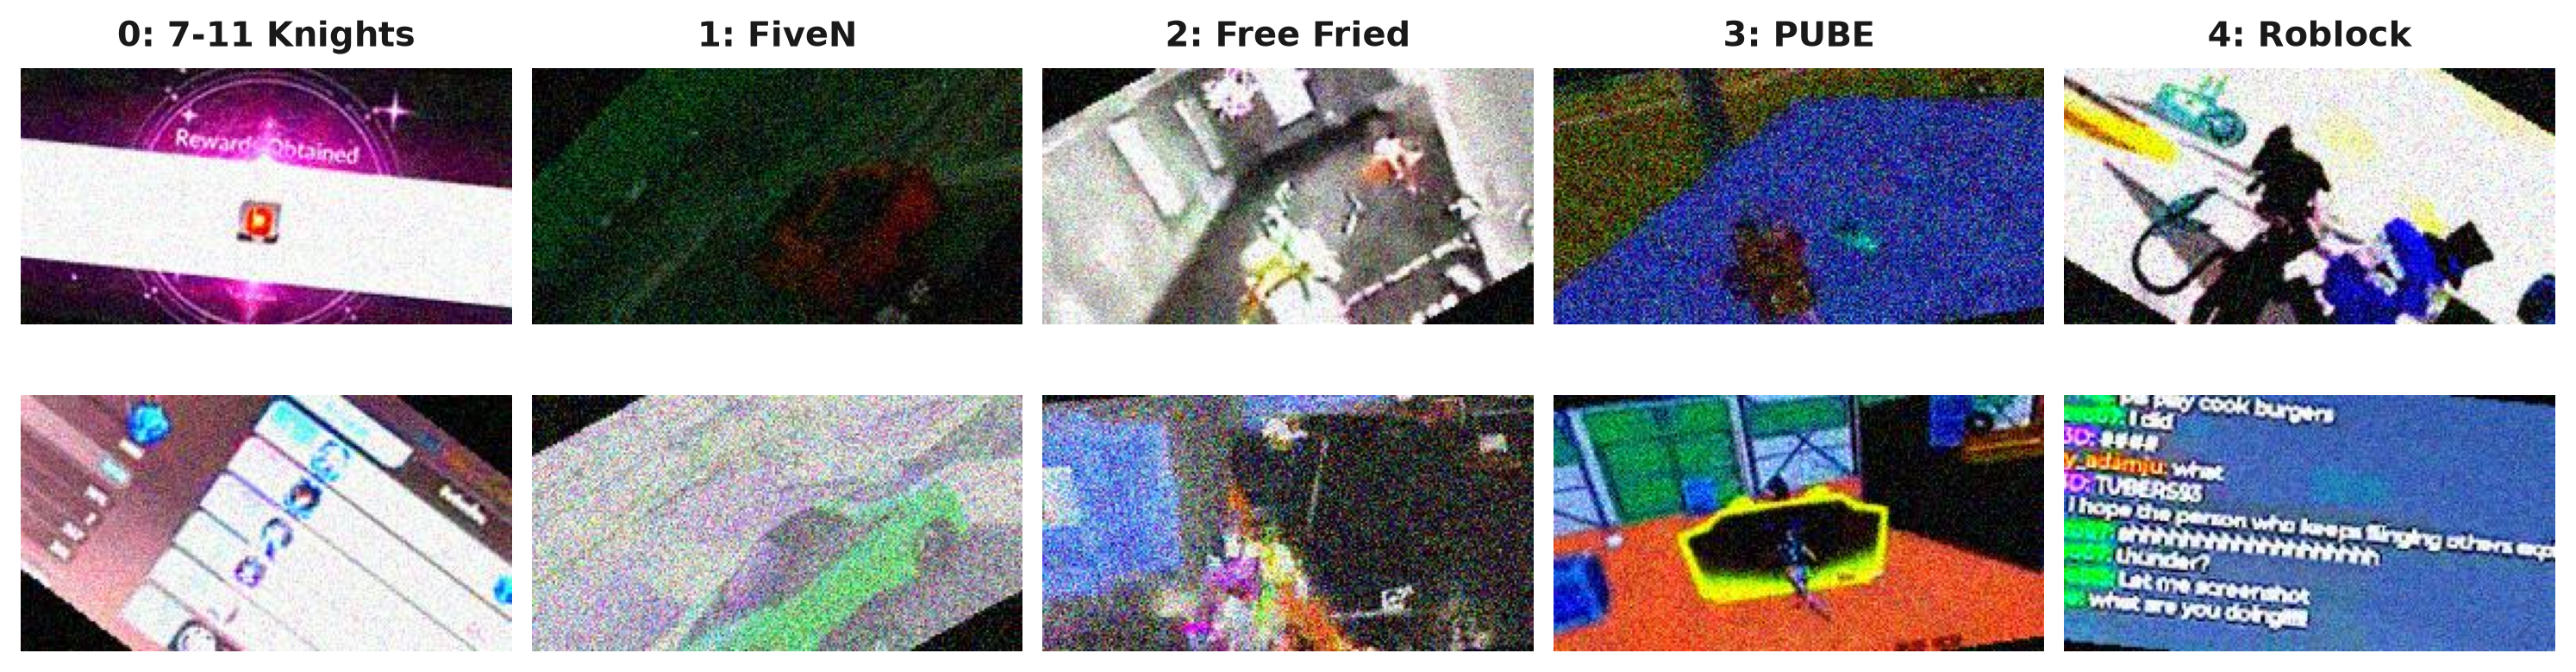
\includegraphics[width=\linewidth,height=0.3\textheight,keepaspectratio]{fig_t4_samples.png}
\caption{Two random training screenshots per title (native $230\times120$). The images are noisy, often rotated with black borders, and contain menus, chat windows and in-game scenes.}
\label{fig:t4-samples}
\end{figure}

\begin{figure}[H]
\centering
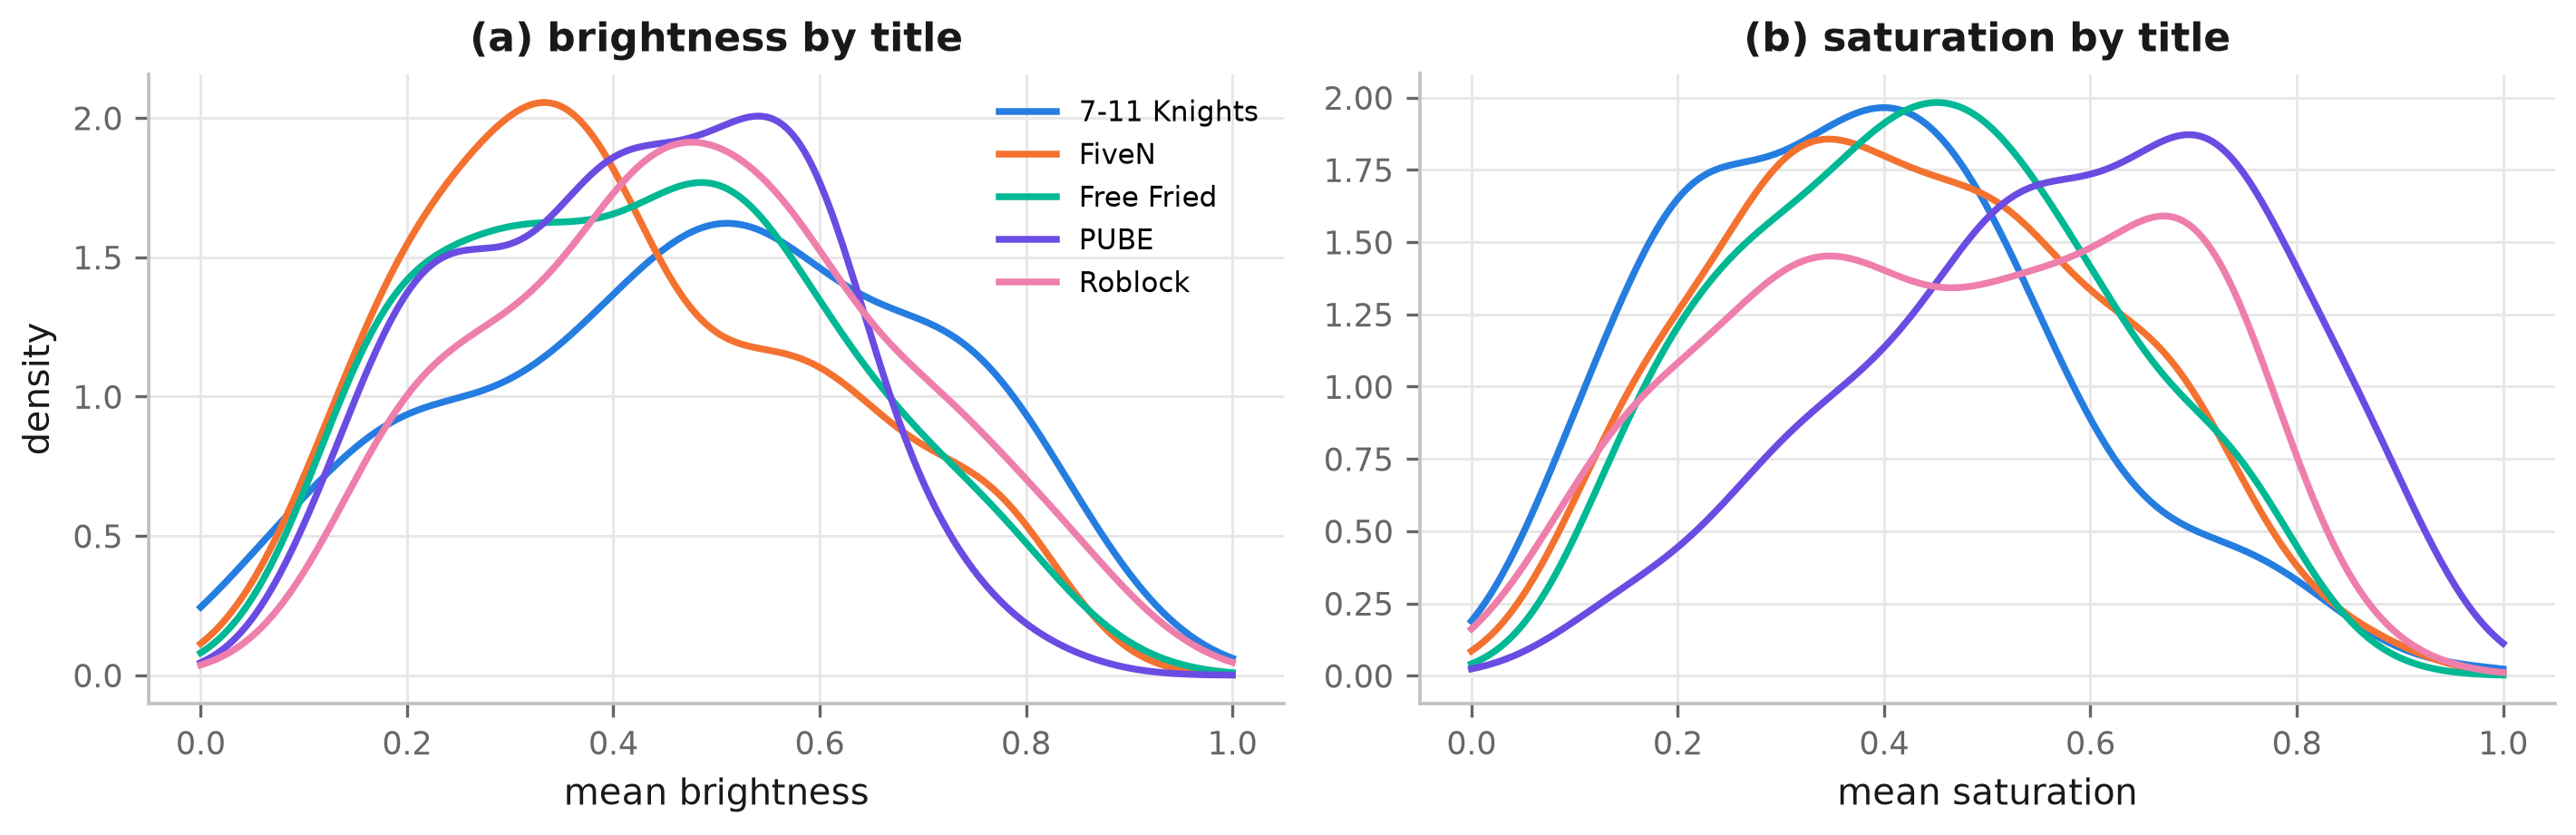
\includegraphics[width=\linewidth,height=0.3\textheight,keepaspectratio]{fig_t4_appearance.png}
\caption{Kernel density of mean brightness and mean saturation by title, 250 random training images per title. The five curves overlap heavily.}
\label{fig:t4-appearance}
\end{figure}

Figure~\ref{fig:t4-samples} shows that the screenshots are small, noisy and varied inside every title, with HUD elements at the sides of a wide frame. Every sampled image has the same size, $230\times120$ (aspect ratio 1.92). Figure~\ref{fig:t4-appearance} shows that brightness and saturation do not separate the titles, so low-level colour statistics are not a usable signal. We decided to resize to a widescreen $224\times416$ input (both sides multiples of the ViT patch size 16) instead of a square crop that would cut away the side HUD, to rely on large pretrained backbones that recognise art style and UI, and to use only generic augmentation (crop, flip, brightness, contrast and saturation jitter).

\paragraph{Near-duplicate scenes.}

\begin{figure}[H]
\centering
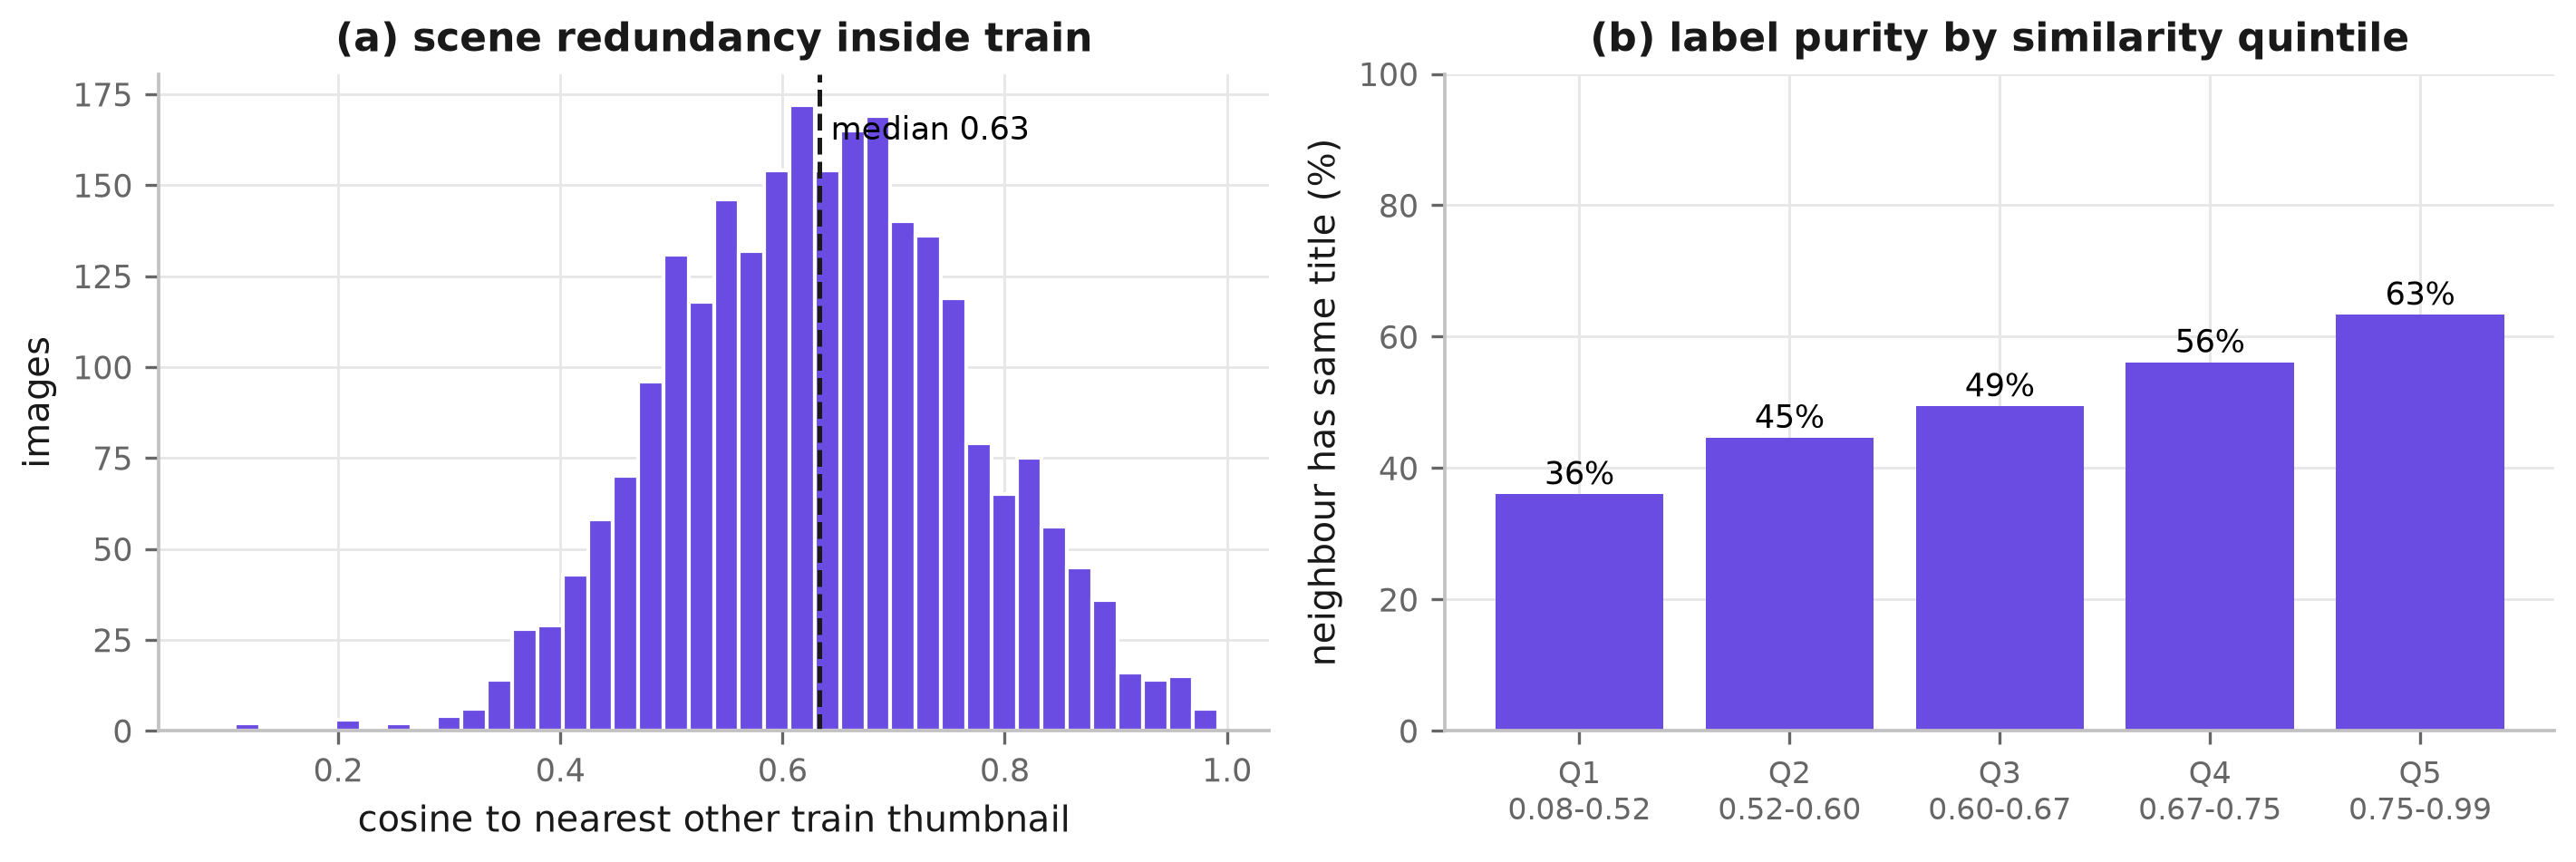
\includegraphics[width=\linewidth,height=0.3\textheight,keepaspectratio]{fig_t4_neardup.png}
\caption{(a) Cosine similarity of each training thumbnail ($28\times16$, 500 per title) to its nearest other training thumbnail. (b) Share of nearest neighbours with the same title, by similarity quintile.}
\label{fig:t4-neardup}
\end{figure}

\begin{figure}[H]
\centering
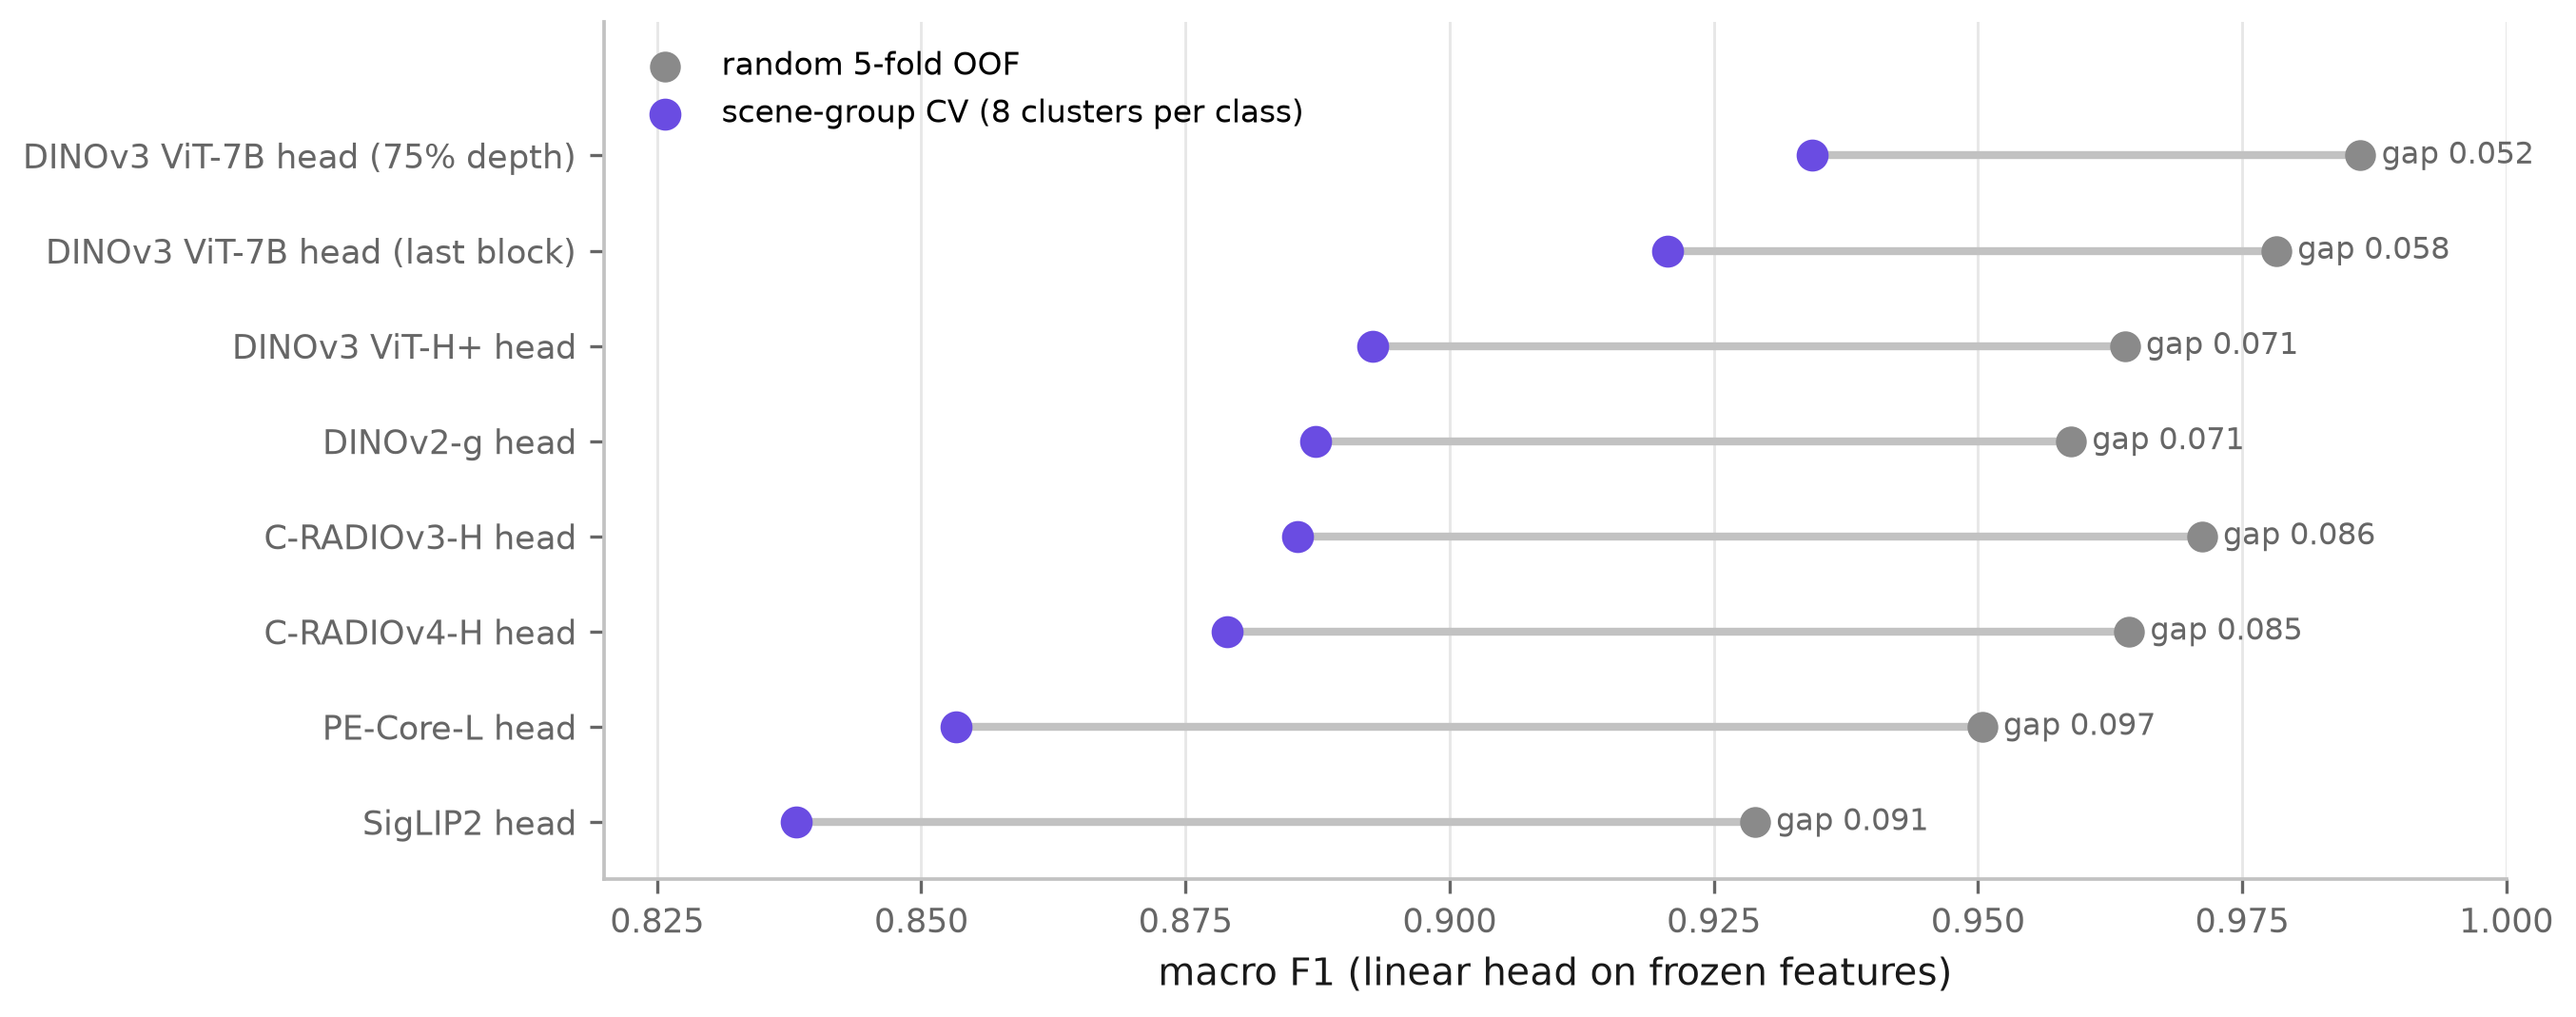
\includegraphics[width=.92\linewidth,keepaspectratio]{fig_t4_cv_gap.png}
\caption{Macro F1 of a linear head on frozen features under random 5-fold CV (grey) and scene-group CV (violet; k-means with 8 clusters per title on frozen features, whole clusters held out). The head variants differ slightly in their views (the random-CV heads used four train views, the scene-group heads two), so gaps are indicative. Every family loses 5--10 points once whole scenes are held out.}
\label{fig:t4-cvgap}
\end{figure}

Even this crude thumbnail descriptor finds many near-duplicates inside the training set (Figure~\ref{fig:t4-neardup}a: median nearest-neighbour cosine 0.63, and 31.4\% of images have a neighbour above 0.70). The label purity of the nearest neighbour rises from 36\% in the least similar quintile to 63\% in the most similar one (Figure~\ref{fig:t4-neardup}b); a $28\times16$ thumbnail is a weak descriptor, so this understates the redundancy that a strong backbone sees. The stronger evidence is Figure~\ref{fig:t4-cvgap}: the same frozen-feature heads that reach 0.93--0.99 under random folds drop to 0.84--0.93 when whole scene clusters are held out. Random folds therefore measure how well a model remembers scenes, not how well it recognises a title in a new scene. We decided to select models, tune ensemble weights and fit calibration on \textbf{scene-grouped folds}.

\subsubsection{Data Preprocessing}

\begin{evidencetable}{EDA evidence and the pipeline decision it motivated (task 4).}{tab:t4-evidence}
Figure~\ref{fig:t4-balance}. About 4:1 class imbalance under macro F1 & Class weights $1/\sqrt{n_k}$ in training; exact uniform-prior logit adjustment at inference using train counts only. \\
Figure~\ref{fig:t4-samples}. Small, noisy, rotated frames with side HUD & Widescreen $224\times416$ input; random-crop, flip and photometric jitter; large pretrained backbones. \\
Figure~\ref{fig:t4-appearance}. Brightness and saturation overlap across titles & No hand-made colour features; photometric jitter only, so the model cannot lean on lighting. \\
Figure~\ref{fig:t4-neardup}. Near-duplicate scenes in train & Scene-grouped stratified folds built from train-only embeddings. \\
Figure~\ref{fig:t4-cvgap}. Random CV overstates every family by 5--10 points & Use scene fold 0 for model choice, depth cut, weights and temperature calibration. \\
\end{evidencetable}

\paragraph{Input pipeline.} Images are loaded once as uint8 tensors at $448\times240$ and resized on the GPU to $224\times416$ with bicubic interpolation and antialiasing, then normalised with the statistics of the backbone (read from \texttt{timm}). At test time we average the log-probabilities of the plain and the horizontally flipped view (test-time augmentation is allowed by the TA).

\paragraph{Augmentation and class weights.} Training uses a random resized crop (area 0.5--1.0, aspect ratio varied by $\pm15\%$), a horizontal flip with probability 0.5, and brightness, contrast and saturation factors drawn from 0.8--1.2. The loss is cross-entropy with label smoothing 0.1 and class weights $\propto 1/\sqrt{n_k}$ (normalised to mean 1).

\paragraph{Scene-grouped folds.} We embed all training images with the frozen ViT-7B (block 30), L2-normalise the embeddings, run k-means with 8 clusters inside each title (40 scene groups), and split the groups with a 5-fold \texttt{StratifiedGroupKFold}. Fold 0 holds 5,113 images from scenes the model never trains on. It is the validation set for every model-selection choice below and the data on which the calibration temperatures are fitted. Nothing in this procedure uses test images.

\subsubsection{Model Design}
\label{sec:t4-design}

The final system is an ensemble of one strong, carefully adapted foundation model (DINOv3 ViT-7B with LoRA) and several diverse companions, combined with weights that depend on how certain each model is for the image at hand. Figure~\ref{fig:t4-pipeline} shows the whole pipeline; Table~\ref{tab:t4-components} lists the components.

\begin{figure*}[t]
\centering
\begin{tikzpicture}[x=1cm,y=1cm]
\tikzset{col/.style={text width=3.3cm}}
% row 1
\node[stage,col] (img) at (0,0) {Train images\\31,546, $230\times120$};
\node[stage,col,fill=\taskcolor{4}!12] (rs) at (3.9,0) {Widescreen $224\times416$\\crop, flip, jitter};
\node[stage,col,fill=\taskcolor{4}!12] (fold) at (7.8,0) {Scene-grouped folds\\8 clusters per title, 5 folds};
\node[stage,col] (cw) at (11.7,0) {Loss: $1/\sqrt{n_k}$ weights, label smoothing 0.1};
\draw[flow] (img) -- (rs);
\draw[flow] (rs) -- (fold);
\draw[flow] (fold) -- (cw);
% row 2: four component groups
\node[model,col,draw=\taskcolor{4},thick] (A) at (0,-3.7) {\textbf{LoRA ViT-7B}\\(DINOv3) cut at 75\% depth, rank 16\\exact soup of 2 adapters\\1- and 2-view heads\\weight 0.52 + 0.25};
\node[model,col] (B) at (3.9,-3.7) {\textbf{Multi-depth LoRA}\\cut at 60\% (blocks 12--23) and at 100\% (blocks 28--39)\\weight 0.04 + 0.04};
\node[model,col] (C) at (7.8,-3.7) {\textbf{Companions}\\fine-tuned ConvNeXt-L/B, EVA02-L/B, ViT-L, DINOv2-L; frozen heads\\weight 0.09};
\node[model,col] (D) at (11.7,-3.7) {\textbf{Joint linear probe}\\10 frozen backbones, 56,576-d, $L_2$-normalised\\weight 0.06};
\coordinate (bus1) at (5.85,-1.75);
\draw[thick,ink!75] (rs.south) -- (rs.south |- bus1);
\draw[thick,ink!75] (0,-1.75) -- (11.7,-1.75);
\foreach \n in {A,B,C,D}{\draw[flow] (\n.north |- bus1) -- (\n.north);}
% row 3: calibration
\node[stage,text width=15cm,fill=\taskcolor{4}!12] (cal) at (5.85,-7.3) {Temperature scaling per model: $\tilde z_m=\log p_m/T_m$, $T_m$ fitted by NLL on scene fold 0 ($T$ from 0.38 for the LoRA soup to 0.68 for the companion group)};
\coordinate (bus2) at (5.85,-6.2);
\draw[thick,ink!75] (0,-6.2) -- (11.7,-6.2);
\foreach \n in {A,B,C,D}{\draw[thick,ink!75] (\n.south) -- (\n.south |- bus2);}
\draw[flow] (bus2) -- (cal.north);
% row 4
\node[stage,text width=4.3cm,fill=\taskcolor{4}!12] (ent) at (1.6,-9.3) {Entropy-weighted pooling\\per-image weight $w_m e^{-H}$};
\node[decision,text width=4.3cm,draw=\taskcolor{4},thick] (pri) at (6.4,-9.3) {Uniform train-prior logit adjustment};
\node[stage,text width=3.3cm,fill=\taskcolor{4}!12] (out) at (11.7,-9.3) {argmax: one title per image};
\draw[flow] (cal.south) -- ++(0,-0.35) -| (ent.north);
\draw[flow] (ent) -- (pri);
\draw[flow] (pri) -- (out);
\node[note] at (5.85,-10.6) {no test statistics enter any weight, temperature or prior};
\end{tikzpicture}
\caption{Task 4 pipeline. Weights are the base weights of the final recipe (they sum to 1). The scene-grouped folds (row 1) choose the model design and fit the temperatures in row 3.}
\label{fig:t4-pipeline}
\end{figure*}

\paragraph{Primary model: LoRA on DINOv3 ViT-7B at 75\% depth.} We truncate the 40-block DINOv3 ViT-7B after block 30 and keep the backbone frozen in bfloat16. LoRA adapters of rank 16 ($\alpha=32$) are attached to every linear layer in the upper blocks, and a head of LayerNorm, dropout 0.1 and a linear layer reads the concatenation of the class token and the mean patch token. The cut at 75\% depth was chosen on scene fold 0 (Section~\ref{sec:t4-eval}). Training uses 3 epochs, batch size 32, AdamW (adapters: learning rate $10^{-4}$, weight decay 0.01; head: $10^{-3}$, 0.05), 5\% warm-up with cosine decay, gradient clipping at 1 and gradient checkpointing. About 10 million parameters are trained. The adapters are trained on the full training set for the final test predictions.

\paragraph{Exact weight-space LoRA soup with dual heads.} Two depth-30 adapters are trained, one on blocks 20--29 and one on blocks 10--29. Averaging the matrices $A$ and $B$ of two independent adapters separately is wrong, because the product $BA$ is not linear in either factor. Instead we concatenate $A_{\text{soup}}=[A_1;A_2]$ and $B_{\text{soup}}=[B_1,B_2]/2$, which gives exactly $B_{\text{soup}}A_{\text{soup}}=\tfrac12(B_1A_1+B_2A_2)$. Two new heads are then refit for 5 epochs on frozen soup embeddings, one on the plain view and one on plain plus flipped views; they are warm-started from the averaged head.

\paragraph{Multi-depth LoRA.} Two further adapters cut the network at 60\% (blocks 12--23 adapted) and at 100\% (blocks 28--39 adapted) of the depth. They are individually weaker on fold 0 but see the image through different layers.

\paragraph{Companions and joint linear probe.} The companion group contains fine-tuned ConvNeXt-Large and ConvNeXt-Base (DINOv3), EVA02-Large and EVA02-Base, DINOv3 ViT-Large and DINOv2-Large, plus frozen-feature linear heads including C-RADIOv3-g. The joint probe concatenates frozen \texttt{[CLS, mean patch]} embeddings of 10 backbone views (DINOv3 ViT-7B at several depths and scales, C-RADIOv3-g, C-RADIOv3-H, C-RADIOv4-H, DINOv2-g, DINOv3 ViT-H+, Web-SSL 1B; 56,576 dimensions). Each backbone block is centred with the training mean and $L_2$-normalised so every family counts equally. One linear layer with weight decay 0.15 is trained for 30 epochs (two seeds), with no hidden layer, so that it cannot memorise scenes.

\begin{table}[H]\centering\small
\caption{Ensemble components and their base weights in the final recipe. $T_m$ is the scene-fold-0 NLL-optimal temperature printed by the submission notebook.}\label{tab:t4-components}
\begin{tabular}{@{}L{.40\linewidth}L{.12\linewidth}L{.12\linewidth}L{.26\linewidth}@{}}
\toprule
\textbf{Component} & \textbf{Weight} & \textbf{$T_m$} & \textbf{Role} \\
\midrule
LoRA soup, 1-view head & 0.52 & 0.380 & main predictor \\
LoRA soup, 2-view head & 0.25 & 0.378 & main predictor \\
LoRA 60\% depth (blocks 12--23) & 0.04 & 0.426 & diversity \\
LoRA 100\% depth (blocks 28--39) & 0.04 & 0.524 & diversity \\
Fine-tuned and frozen companions & 0.09 & 0.677 & tie-breaking \\
10-backbone joint linear probe & 0.06 & 0.454 & scene-robust consensus \\
\bottomrule
\end{tabular}
\end{table}

\paragraph{Temperature calibration and entropy-weighted pooling.} Models trained with label smoothing 0.1 produce compressed log-probabilities, which is why the LoRA temperatures are about 0.38 while the unsmoothed companions need about 0.68. Dividing each model's log-probabilities by its own $T_m$ puts them on a common scale. For an image $x$, the weight of model $m$ is $w_m(x)=w_m\,\exp(-H(\tilde p_m(x)))$, where $H$ is the Shannon entropy of the calibrated probabilities. On confident images the LoRA soup dominates; when the soup is uncertain, the other families get more say. The pooled calibrated logits are $\sum_m w_m(x)\tilde z_m$.

\paragraph{Exact uniform-prior logit adjustment.} Macro F1 is best served by a decision rule for a uniform class prior. We subtract $\big(\sum_m w_m(x)/T_m\big)\log\pi_{\text{train}}$ from the pooled logits, where $\pi_{\text{train}}$ is the class frequency of the training set (Figure~\ref{fig:t4-balance}). This is a fixed vector computed from training labels only; the TA confirmed that such a prior may be applied to the test set as a fixed value. The prediction is the argmax of the result.

\subsubsection{Evaluation and Results}
\label{sec:t4-eval}

\paragraph{Validation.} Because random folds hide the scene shift (Figure~\ref{fig:t4-cvgap}), all model choices use scene fold 0 (5,113 images, never seen in training). Table~\ref{tab:t4-fold0} shows how each design step changed fold-0 errors.

\begin{table}[H]\centering\small
\caption{Scene fold 0 (5,113 images). The final row is the submission notebook's printed result.}\label{tab:t4-fold0}
\begin{tabular}{@{}L{.56\linewidth}L{.16\linewidth}L{.14\linewidth}@{}}
\toprule
\textbf{Model} & \textbf{Macro F1} & \textbf{Errors} \\
\midrule
ConvNeXt-S DINOv3 fine-tune (scene-fold proxy) & 0.9728 & --- \\
Frozen ViT-7B head, last block & 0.9749 & --- \\
Frozen ViT-7B head, 75\% depth & 0.9834 & --- \\
LoRA ViT-7B, 75\% depth, averaged head & 0.99115 & 42 \\
LoRA, depth 30 on blocks 10--29 & 0.99172 & 40 \\
Exact soup, refit head & 0.9937 & 30 \\
Exact soup, refit head, with train prior & 0.99467 & 21 \\
\textbf{Final ensemble (sub\_v90f recipe)} & \textbf{0.99482} & \textbf{21} \\
\bottomrule
\end{tabular}
\end{table}

\begin{figure}[H]
\centering
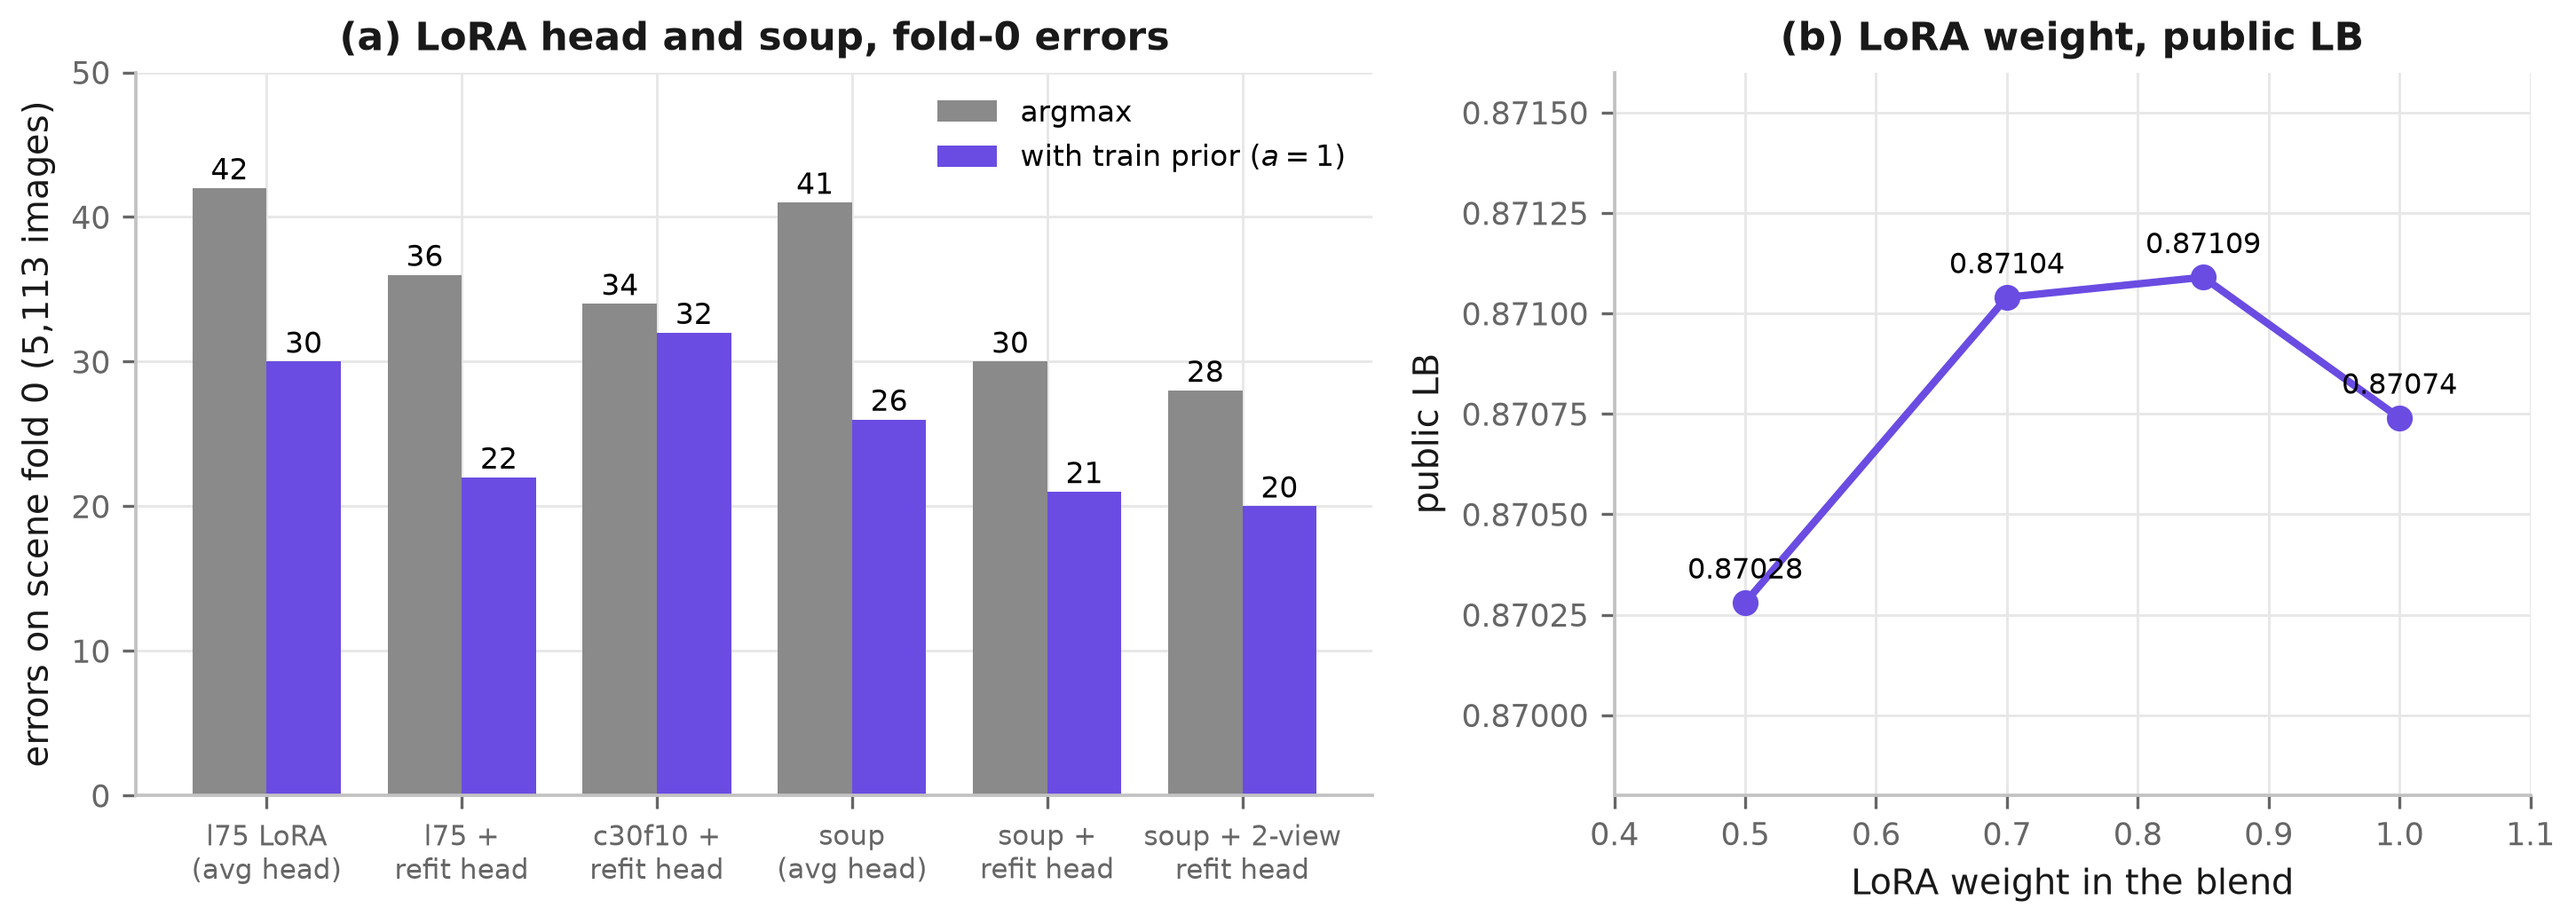
\includegraphics[width=\linewidth,height=0.32\textheight,keepaspectratio]{fig_t4_lora_soup.png}
\caption{(a) Errors on scene fold 0 for the single LoRA models, the soup and the heads, before and after the train prior. (b) Public leaderboard against the LoRA weight in the blend (the rest is a frozen-feature blend). The head refit and the prior remove most errors; the LoRA weight has a flat top near 0.7--0.85.}
\label{fig:t4-lora-soup}
\end{figure}

\paragraph{Leaderboard.} The submission \texttt{sub\_v90f\_entropy\_dualhead\_md.csv} scored a public LB of \textbf{0.87351} (1st). It differs from earlier files only in Task 4. Table~\ref{tab:t4-milestones} lists milestones of the Task 4 work (the public score is the average over five tasks, so a Task 4 change of $\Delta$ F1 moves it by about $0.2\Delta$ if the tasks are weighted equally, which we assume but did not verify).

\begin{table}[H]\centering\small
\caption{Public LB milestones (all other tasks fixed within a pair of rows). Rule-excluded files (test-derived EM prior) are left out.}\label{tab:t4-milestones}
\begin{tabular}{@{}L{.12\linewidth}L{.58\linewidth}L{.2\linewidth}@{}}
\toprule
\textbf{File} & \textbf{Task 4 recipe} & \textbf{Public LB} \\
\midrule
v25a & ConvNeXt-T + EVA02-S, realigned to the new test order & 0.85787 \\
v28 & + ConvNeXt-S DINOv3 & 0.85906 \\
v30 & equal 4 fine-tuned models, adds ConvNeXt-B & 0.86169 \\
v32 & + frozen-feature heads, 50/50 with fine-tuned models & 0.86430 \\
v74b\_clean & full-train fine-tuned set + frozen ViT-7B head, no EM & 0.86812 \\
v79c\_clean & + LoRA ViT-7B at weight 0.85 & 0.87109 \\
v81b & + uniform train-prior adjustment & 0.87307 \\
v85a & LoRA slot = exact soup with refit head & 0.87346 \\
\textbf{v90f} & + temperature, entropy-weighted pooling, multi-depth & \textbf{0.87351} \\
\bottomrule
\end{tabular}
\end{table}

Most of the gain came from three steps: more and different fine-tuned backbones (+0.0064 from v25a to v32), the LoRA ViT-7B (+0.0030 from v74b\_clean to v79c\_clean) and the train prior (+0.0020). The last two steps (soup, calibrated entropy pooling) add 0.0004 and 0.00005, which is within the noise of a public leaderboard. We kept them because fold 0 supports them and they do not use any test statistic.

\paragraph{Decision log.} Figure~\ref{fig:t4-decision-log} shows every Task 4 experiment with the change in public LB, coloured by whether we kept it, dropped it or excluded it for rule reasons; the rows are in \texttt{data/decision\_log\_t4.csv}.

\begin{figure}[p]
\centering
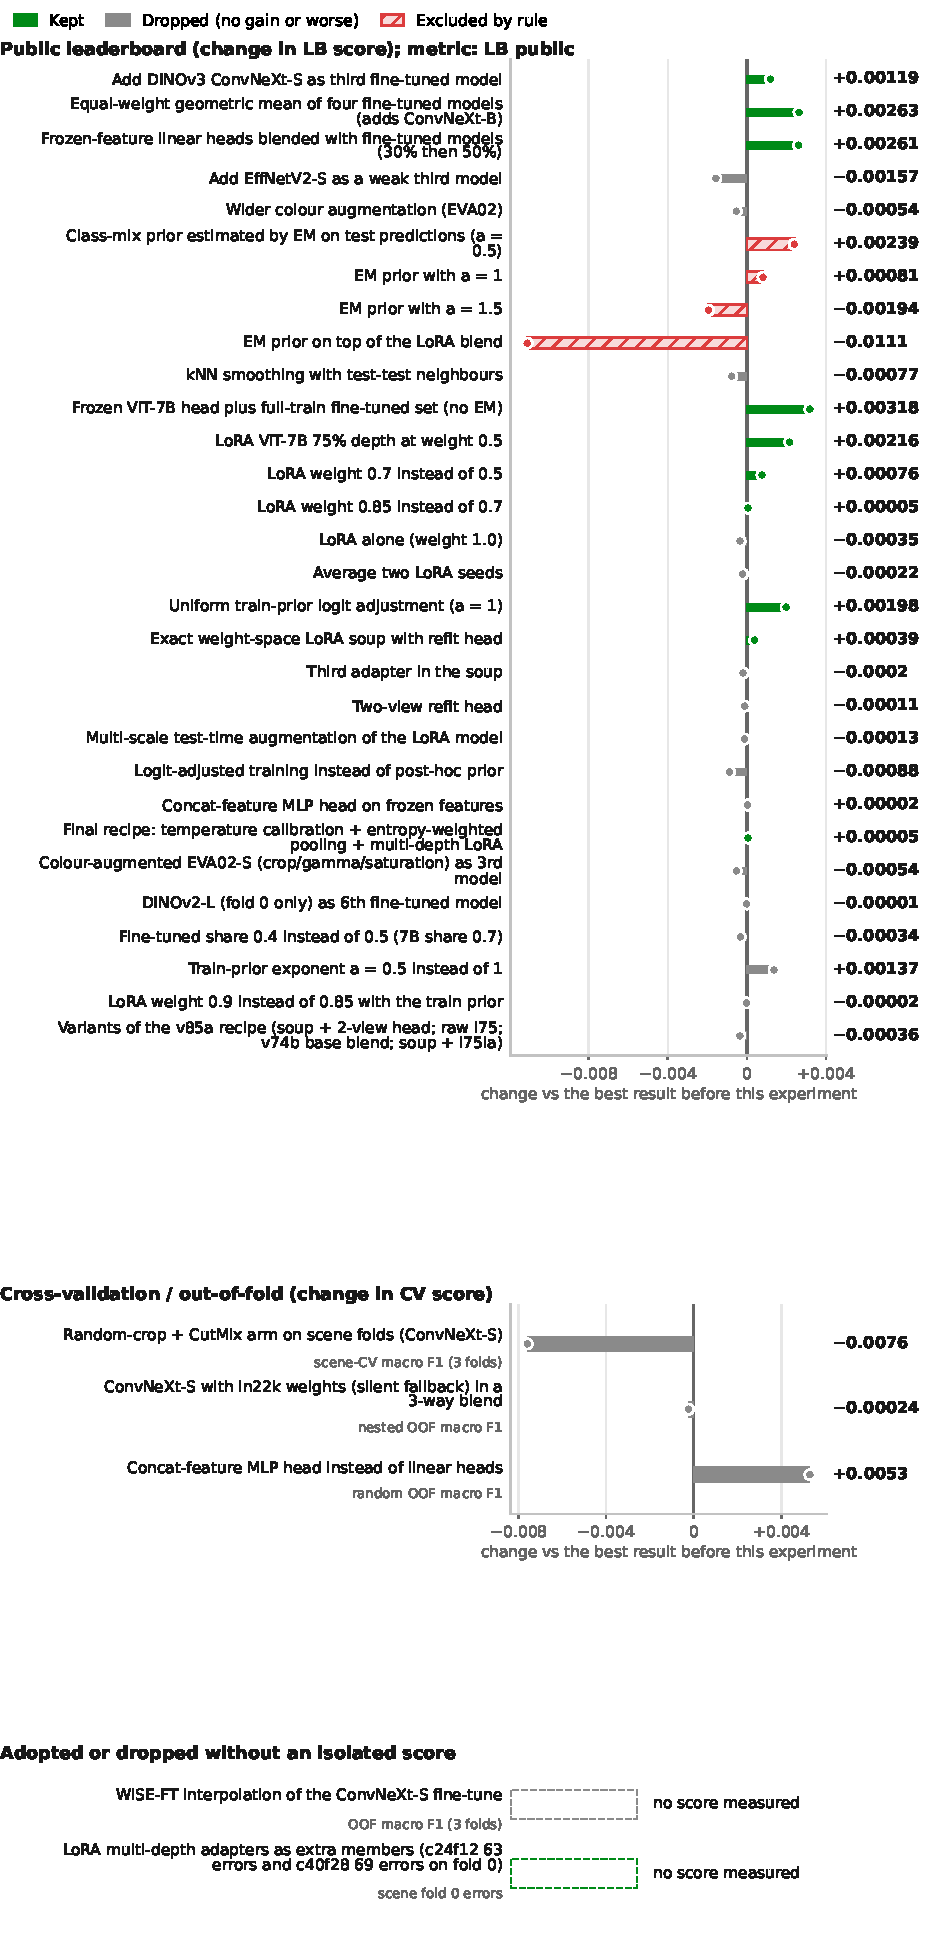
\includegraphics[width=\linewidth,height=0.85\textheight,keepaspectratio]{decision_log_t4.pdf}
\caption{Task 4 decision log: change in public LB per experiment, kept versus dropped versus rule-excluded. Green = kept, grey = dropped, red hatched = excluded by the competition rules.}
\label{fig:t4-decision-log}
\end{figure}

\subsubsection{Insights from Model Behaviour}

\paragraph{Where the model errs.} Before the prior correction, 22 of the 41 errors counted for the single LoRA model on fold 0 (Table~\ref{tab:t4-fold0} gives 42 for the final training run) were FiveN or Free Fried images predicted as 7-11 Knights, the largest training class (prior 0.394). The model had learned the training class mix. The uniform-prior adjustment removes the bias directly: errors of the soup with refit head fell from 30 to 21 on fold 0 (Figure~\ref{fig:t4-lora-soup}a), and the public LB rose by 0.0020 when the same adjustment was added to the LoRA blend. No fold-0 error had a confidence above 0.9.

\paragraph{Intermediate depth beats the last block.} A linear head on the 75\%-depth features of the ViT-7B reaches 0.9834 on fold 0 and a head on the last block reaches 0.9749 (Table~\ref{tab:t4-fold0}); under random folds the gap is smaller (0.9862 against 0.9782). Intermediate features carry more transferable scene content than the final block, and the scene folds make that visible while random folds do not. Fine-tuning adapters (LoRA) on top of the 75\% features then lifts fold 0 to 0.9912 for a single model.

\paragraph{Fine-tuning and frozen features are complementary.} On scene folds a fine-tuned ConvNeXt-S beat every frozen head, yet blending the two at about 50/50 beat either alone (0.9697 against 0.9635 for the fine-tuned model alone in our proxy study). This is why the final recipe keeps the joint linear probe and the frozen heads inside the ensemble even though the LoRA soup carries 77\% of the base weight.

\paragraph{Behaviour on the shifted test set (leaderboard observation).} Random-fold OOF ranked models poorly against the public leaderboard: it underrated larger backbones and gave no sign of the benefit of frozen features (Task 4 changes with OOF gain $+0.0005$ produced $+0.0012$ on the LB). We learned this from leaderboard results, not from inspecting test images, and we did not use test statistics to choose any final setting. Under the assumption of equal task weights and Task 1--3 and 5 scores close to their validation values, the public LB 0.87351 implies a Task 4 macro F1 of about 0.98 on the test set (our own estimate, not an official number), against 0.995 on scene fold 0, so the test set is harder than fold 0 and there is still headroom.

\subsubsection{Common Mistakes and Failed Experiments}

\paragraph{Test-derived class prior (rule issue).} After the data re-release the predicted test mix differed strongly from the training mix. We estimated the test class prior with EM on our own test predictions and corrected the probabilities; this was worth $+0.0032$ on the public LB. The TA ruled on 16 November that estimating the class mix from test predictions is the same as pseudo-labelling and is \textbf{not allowed}, while a prior computed from train labels and applied as a fixed value is allowed. We replaced the EM prior by the uniform train prior (exponent $a=1$, justified by macro F1, not tuned), which scored even higher once the LoRA model was in (+0.0020 over the same file without a prior; the EM prior on the LoRA blend scored $-0.0111$). Every EM file is rule-excluded in Figure~\ref{fig:t4-decision-log}.

\paragraph{Choices driven by test statistics.} Early frozen heads were trained with extra darkened and saturated copies of the training images, because we had compared brightness and saturation between train and test images. The TA ruled that comparing train and test image statistics to choose augmentation or validation is a leak. The final heads use plain and flipped views only, and the scene-grouped validation is now justified by training-set evidence only (Figures~\ref{fig:t4-neardup} and \ref{fig:t4-cvgap}). The wider colour augmentation that we tried on the same suspicion scored $-0.00054$.

\paragraph{Random-fold OOF.} The first ensembles were chosen by random-fold OOF (about 0.99), which looks excellent but ranks models poorly; the multilayer-perceptron head on frozen features gained on OOF and on hard rows and gave $+0.00002$ on the leaderboard (Figure~\ref{fig:t4-decision-log}).

\paragraph{Wrong row order after the data re-release.} On 12 November the organisers regenerated the data and the new \texttt{test.csv} listed the images in a different order. Our old predictions were still aligned to the old order, which matched the new one only at chance (21\%); Task 4 therefore scored at chance on the leaderboard until we realigned the predictions by file name, after which the public LB rose by 0.1375. Lesson: join predictions to the test list by \texttt{file\_name}, never by position, and test with a probe file.

\paragraph{Experiments that did not help.} Moving the final recipe forward from the LoRA model, none of the following improved the public score: kNN smoothing with test-test neighbours ($-0.00077$), EM exponent 1.5 ($-0.00194$), an equal-weight blend with the weak EffNetV2-S ($-0.00157$), logit-adjusted training instead of the post-hoc prior ($-0.00088$), averaging two LoRA seeds ($-0.00022$), a third adapter in the soup ($-0.0002$), the two-view refit head ($-0.00011$), multi-scale test-time augmentation ($-0.00013$), and a WiSE-FT interpolation (no movement of test predictions toward the frozen heads; not submitted). Weight tuning (LoRA share, FT/frozen share) was closed once the curve flattened (Figure~\ref{fig:t4-lora-soup}b).

\paragraph{Limitations.} Fold 0 is a single scene fold, so 21 errors versus 20 or 22 is within noise; we resisted tuning on such differences. The final ensemble weights were set by hand and by the public leaderboard history, not by a nested search, and the full-train models have no out-of-fold prediction of their own. The intermediate steps between v85a and v90f (v88--v91) are not documented in our log; \todo{list v88--v91 results if the team wants a complete ablation of the calibration and entropy-pooling steps.}

\subsubsection{Domain Interpretation and Business Impact}

The course scenario for Task 4 gives three operational pains: about 2,000 support tickets per day with screenshots that take 10 or more minutes each to route, 50,000+ campaign screenshot submissions of which only 3\% can be checked by hand, and 100,000+ gameplay images posted weekly that cannot be auto-tagged for contests, moderation or trend tracking. If the triage of the tickets alone took 10 minutes each, it would cost more than 330 person-hours per day, so an automated title detector pays off mainly by removing this routing step and by making full verification of campaign submissions possible.

The cost of an error depends on the use. For ticket routing, a wrong title sends the ticket to the wrong specialist queue; for campaigns, a false match may reward a screenshot from another game. A deployed system should therefore send low-confidence predictions to a human. Our model is well calibrated per model (temperatures are fitted on held-out scenes), but the entropy-weighted output is not a calibrated probability, so a review threshold should be set on a labelled validation set of new scenes. On the competition test set the system is less certain than on fold 0 (leaderboard-implied macro F1 near 0.98 against 0.995), which warns that new maps or new art styles will lower accuracy.

Deployment caveats: (i) the class mix of live traffic differs from the training mix, and our uniform-prior rule assumes macro-F1-style equal importance of the titles; for ticket volume the real prior should be used instead. (ii) The ViT-7B with adapters and the many companions need a large GPU; a production system would distil the ensemble into one smaller model or keep only the LoRA soup. \todo{measure inference time per image for the LoRA soup and for the full ensemble.} (iii) Screenshots from new game updates will be new scenes, so the model should be re-validated with scene-grouped folds after each content release.

\end{document}
